%%%%%%%%%%%%%%%%%%%%%%%%%%%%%%%%%%%%%%%%%
% Beamer Presentation
% LaTeX Template
% Version 1.0 (10/11/12)
%
% This template has been downloaded from:
% http://www.LaTeXTemplates.com
%
% License:
% CC BY-NC-SA 3.0 (http://creativecommons.org/licenses/by-nc-sa/3.0/)
%
%%%%%%%%%%%%%%%%%%%%%%%%%%%%%%%%%%%%%%%%%

%----------------------------------------------------------------------------------------
%	PACKAGES AND THEMES
%----------------------------------------------------------------------------------------

\documentclass{beamer}

\mode<presentation> {

% The Beamer class comes with a number of default slide themes
% which change the colors and layouts of slides. Below this is a list
% of all the themes, uncomment each in turn to see what they look like.

%\usetheme{default}
%\usetheme{AnnArbor}
%\usetheme{Antibes}
%\usetheme{Bergen}
%\usetheme{Berkeley}
%\usetheme{Berlin}
%\usetheme{Boadilla}
%\usetheme{CambridgeUS}
%\usetheme{Copenhagen}
%\usetheme{Darmstadt}
%\usetheme{Dresden}
%\usetheme{Frankfurt}
%\usetheme{Goettingen}
%\usetheme{Hannover}
%\usetheme{Ilmenau}
%\usetheme{JuanLesPins}
%\usetheme{Luebeck}
\usetheme{Madrid}
%\usetheme{Malmoe}
%\usetheme{Marburg}
%\usetheme{Montpellier}
%\usetheme{PaloAlto}
%\usetheme{Pittsburgh}
%\usetheme{Rochester}
%\usetheme{Singapore}
%\usetheme{Szeged}
%\usetheme{Warsaw}

% As well as themes, the Beamer class has a number of color themes
% for any slide theme. Uncomment each of these in turn to see how it
% changes the colors of your current slide theme.

%\usecolortheme{albatross}
%\usecolortheme{beaver}
%\usecolortheme{beetle}
%\usecolortheme{crane}
%\usecolortheme{dolphin}
%\usecolortheme{dove}
%\usecolortheme{fly}
%\usecolortheme{lily}
%\usecolortheme{orchid}
%\usecolortheme{rose}
%\usecolortheme{seagull}
%\usecolortheme{seahorse}
%\usecolortheme{whale}
%\usecolortheme{wolverine}

%\setbeamertemplate{footline} % To remove the footer line in all slides uncomment this line
%\setbeamertemplate{footline}[page number] % To replace the footer line in all slides with a simple slide count uncomment this line

%\setbeamertemplate{navigation symbols}{} % To remove the navigation symbols from the bottom of all slides uncomment this line
}

\usepackage{graphicx} % Allows including images
\usepackage{booktabs} % Allows the use of \toprule, \midrule and \bottomrule in tables
\usepackage{graphicx}

%----------------------------------------------------------------------------------------
%	TITLE PAGE
%----------------------------------------------------------------------------------------

\title[Evolving Part-DNA Substructures]{The Automated Modeling and Optimization of Part DNA Substructures Employing Evolutionary Computation} % The short title appears at the bottom of every slide, the full title is only on the title page

\author{Daniel Tauritz, Bailey Eversmeyer} % Your name
\institute[MST] % Your institution as it will appear on the bottom of every slide, may be shorthand to save space
{
Missouri University of Science and Technology \\ % Your institution for the title page
\medskip
\textit{tauritzd@mst.edu, rbe62d@mst.edu} % Your email address
}
\date{\today} % Date, can be changed to a custom date

\begin{document}

\begin{frame}
\titlepage % Print the title page as the first slide
\end{frame}

\begin{frame}
\frametitle{Overview} % Table of contents slide, comment this block out to remove it
\tableofcontents % Throughout your presentation, if you choose to use \section{} and \subsection{} commands, these will automatically be printed on this slide as an overview of your presentation
\end{frame}

\section{Part-DNA}

\begin{frame}
\frametitle{Part-DNA Overview}
Goals:
\begin{itemize}
\item Model and map the flow of goods and components through a system
\item Track the changes to components over time
\item Help identify relationships between components
\item Makes analyzing the system easier
\end{itemize}
\end{frame}

\begin{frame}
\frametitle{How We Fit into the Part-DNA Model}
\begin{enumerate}
\item Choose a substructure of the Part-DNA Model\pause
\item Gather data on input-output component transformations\pause
\item Model the transformations of components through the section\pause
\item Gather data on possible input components\pause
\item Test new input combinations to map Pareto Trade-Off surface
\end{enumerate}
\end{frame}

\begin{frame}
\frametitle{Our Model Concept}
\begin{figure}
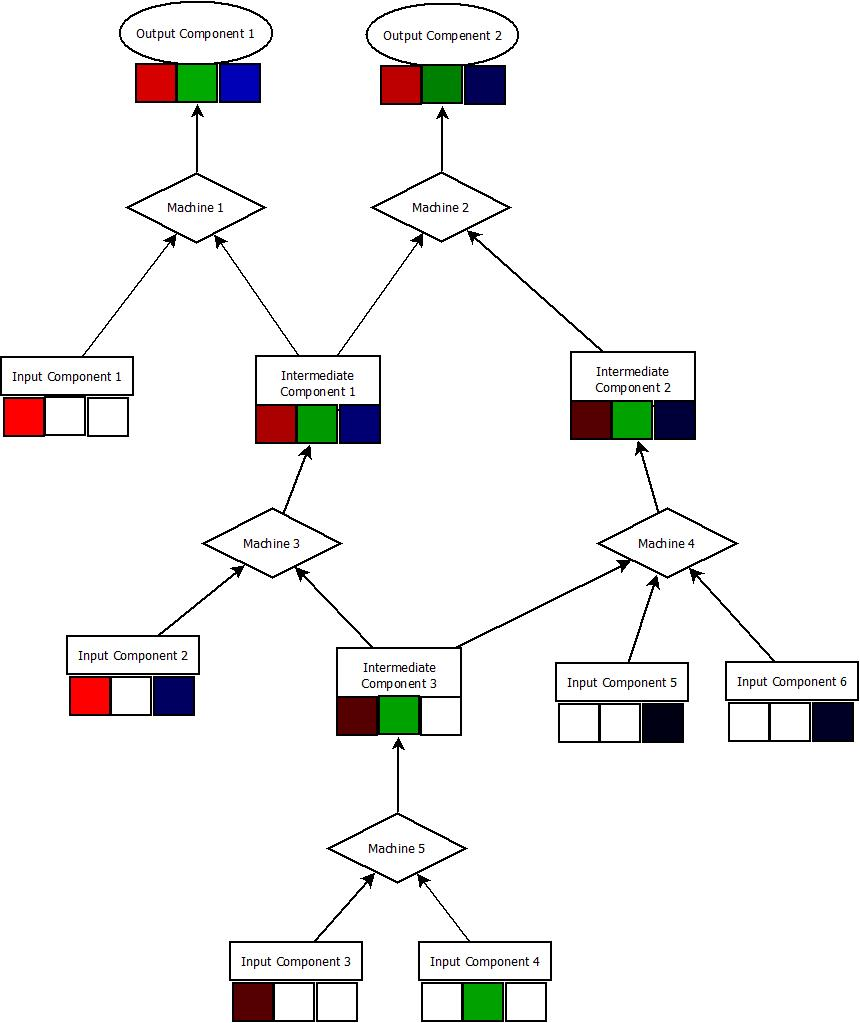
\includegraphics[width=0.5\linewidth]{BaseModel.jpeg}
\end{figure}
\end{frame}

\section{Evolutionary Computation Strategies}

\subsection{Genetic Programming}

\begin{frame}
\frametitle{Genetic Programming (GP)}

\end{frame}

\subsection{Evolutionary Algorithms}

\begin{frame}
\frametitle{Evolutionary Algorithms (EAs)}

\end{frame}

\begin{frame}
\frametitle{Multi-Objective EAs (MOEAs)}

\end{frame}

\section{Application of EC Strategies}

\begin{frame}
\frametitle{GP Section}
\begin{figure}
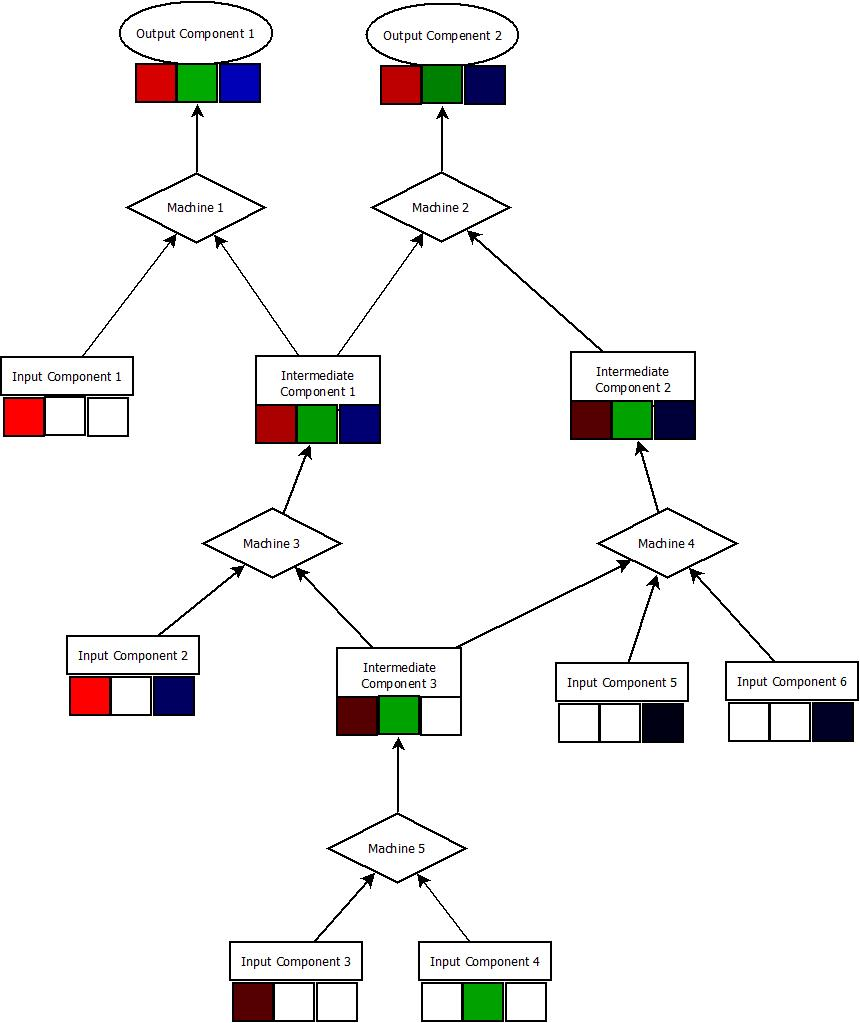
\includegraphics[width=0.5\linewidth, trim={6cm 0 8.1cm 17.1cm},clip]{BaseModel.jpeg}
\end{figure}
\end{frame}

\begin{frame}
\frametitle{GP Process}
Given a dataset of input-output combinations

For each output attribute:
\begin{itemize}
\item Generate population of randomized functions from the input domain\pause
\item Assign fitness value based on error across the dataset\pause
\item Explore the function domain through recombination and mutation of functions
\end{itemize}
Repeat for each transformation object
\end{frame}

\begin{frame}
\frametitle{MOEA Section}
With the modeled functions in hand, we apply our MOEA to the whole process to optimize for the output parameters
\begin{figure}
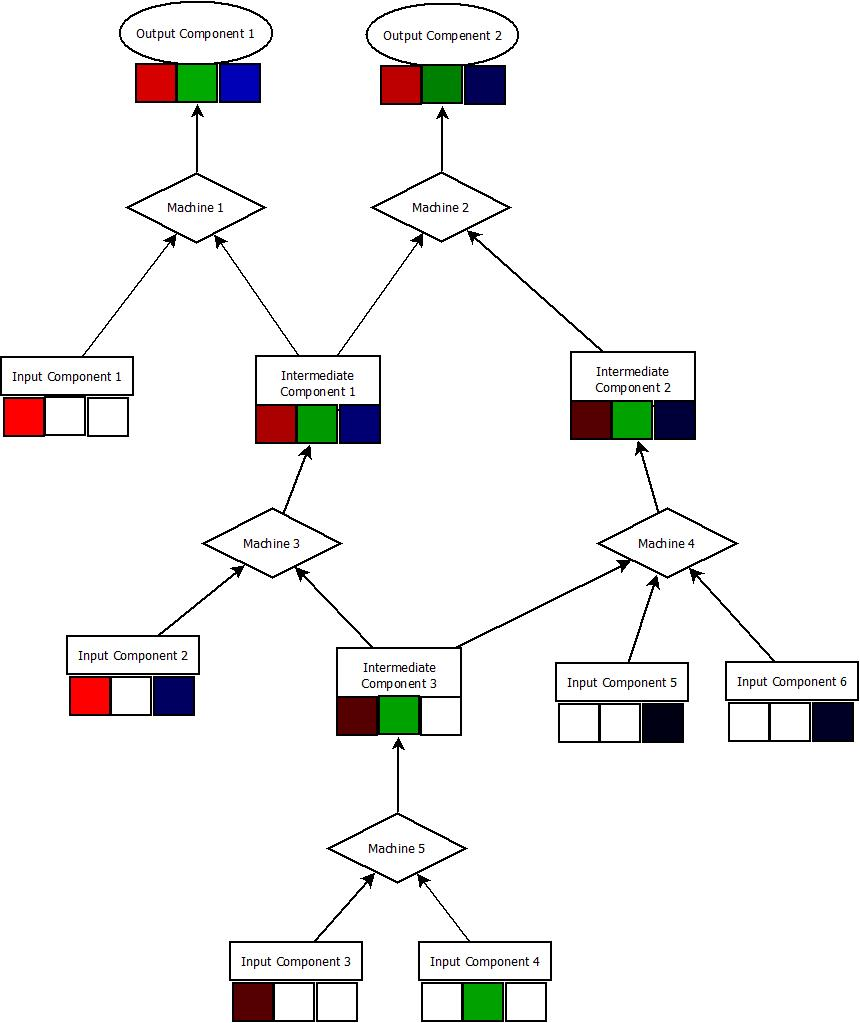
\includegraphics[width=0.4\linewidth]{BaseModel.jpeg}
\end{figure}
\end{frame}

\begin{frame}
\frametitle{MOEA Process}
Given a dataset of possible inputs and desired outputs:
\begin{itemize}
\item Generate population of randomly chosen inputs\pause
\item Simulate the system with each input combination\pause
\item Assign fitness values for Accuracy and Affordability\pause
\item Rate solutions based on their Pareto score\pause
\item Explore the input combination domain through recombination and mutation of solutions
\end{itemize}
End with a selection of Pareto Optimal solutions, and associated trade-off information.
\end{frame}

\begin{frame}
\frametitle{Example Pareto Front over Time}
\begin{figure}
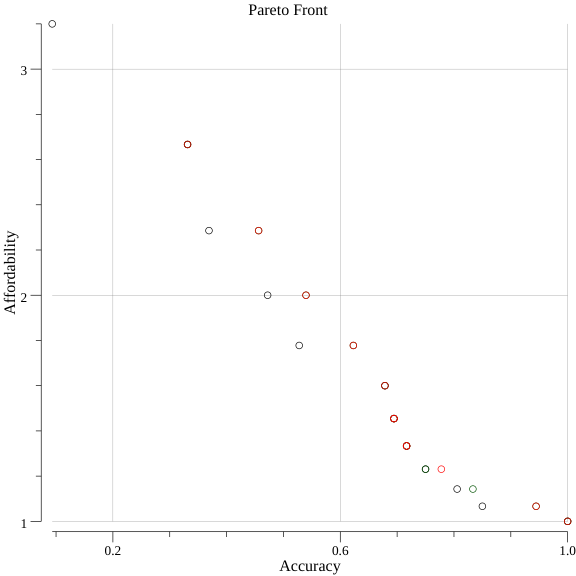
\includegraphics[width=0.6\linewidth]{points.png}
\end{figure}
\end{frame}

\begin{frame}
\Huge{\centerline{Questions?}}
\end{frame}

\end{document}